\section{CUDA 课程项目二：线程束 ID（Warp ID）}

在前一个项目中，我们研究了块 ID（Block ID）和线程 ID（Thread ID）。本章将研究第三层级——\textbf{线程束 ID}（Warp ID）。

\subsection{Warp ID 概念}

每个 GPU 应用程序包含网格（Grid），网格包含块（Block），块包含线程束（Warp），每个线程束由 32 个线程组成。这就是 CUDA 程序中的四级软件层级结构。

\begin{figure}
    \centering
    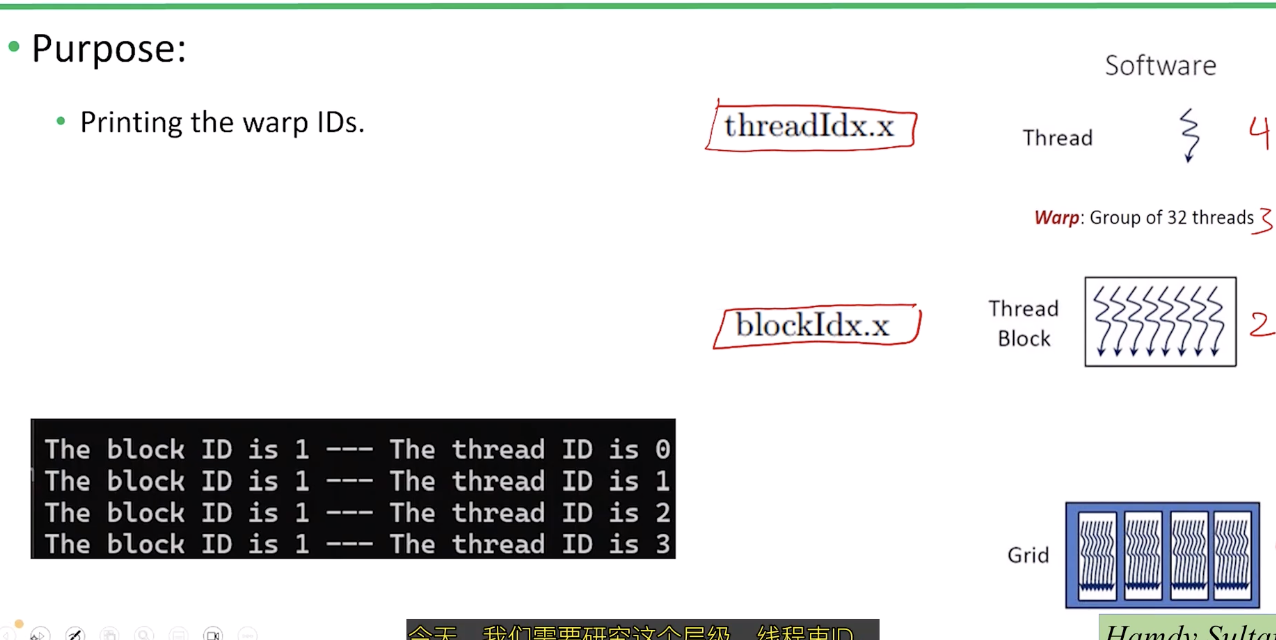
\includegraphics[width=0.75\linewidth]{resources/cuda-072.png}
    \caption{}
    \label{fig:placeholder}
\end{figure}

前文已经学习了如何打印线程 ID（X、Y、Z 三个维度）和块 ID。本章的目标是计算并打印线程束 ID。这里的关键问题是：CUDA 中\textbf{没有}预定义变量直接提供线程束 ID 值，需要我们自行计算。

\subsection{计算 Warp ID}

已知每个线程束由 32 个线程组成，如果每个块有 128 个线程，则每块有 $128 / 32 = 4$ 个线程束。

计算线程束 ID 的方法如下：声明变量 \texttt{WarpID}，将其初始化为 0，然后令其等于当前线程的线程 ID 除以 32。每个线程的线程 ID 不同，除法运算后得到该线程所属的线程束 ID。

\begin{figure}
    \centering
    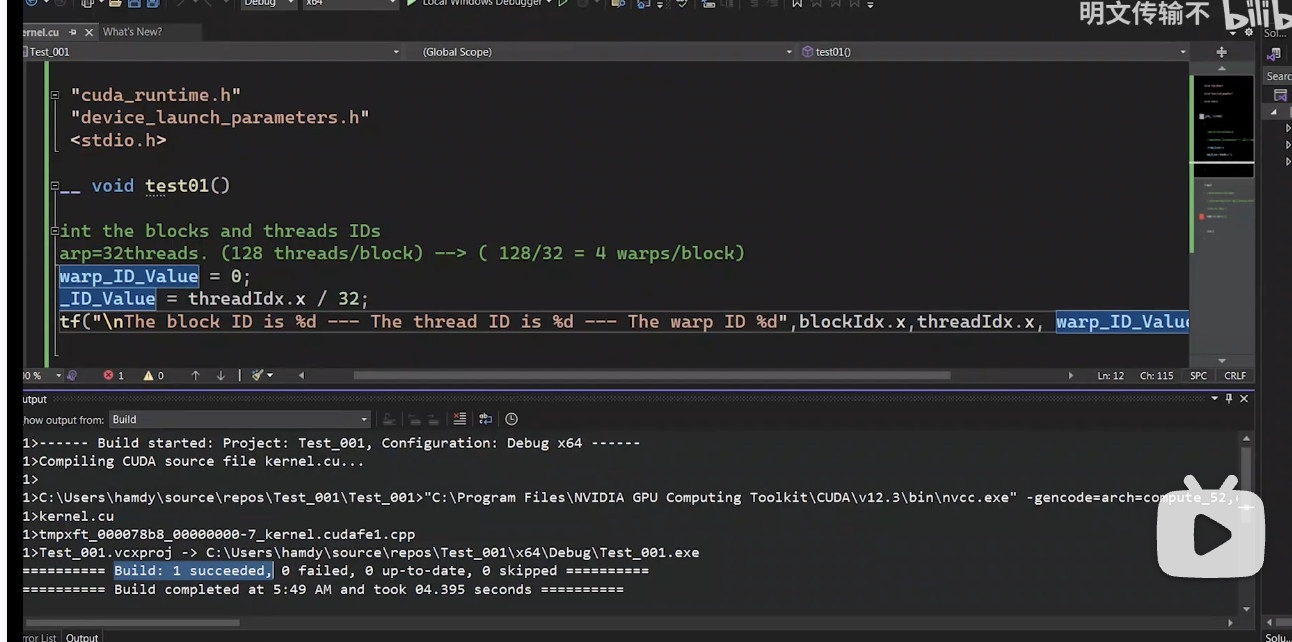
\includegraphics[width=0.75\linewidth]{resources/cuda-073.png}
    \caption{}
    \label{fig:placeholder}
\end{figure}

编译并运行后，可以看到输出结果。首先关注块 ID：当只有 1 个块时，块 ID 始终为 0。线程 ID 从 0 开始（由于并行执行，输出顺序不一定连续），最大值为 127。线程束 ID 从 0 开始，共有 4 个（0、1、2、3），每个线程束包含 32 个线程——线程束 0 包含线程 ID 0 到 31，线程束 3 包含线程 ID 96 到 127。

此时项目中有 1 个块、4 个线程束，每个线程束由 32 个线程组成。计算线程束 ID 还有其他方法（例如使用取模运算），读者可以自行探索。

\subsection{多块场景下的 Warp ID}

将每块线程数改为 64，则每块有 $64 / 32 = 2$ 个线程束。如果同时将块数改为 2，每块的线程束数仍为 2（因为未改变每块线程数），但整个 GPU 上的总线程束数变为 $2 \times 2 = 4$。

\begin{figure}
    \centering
    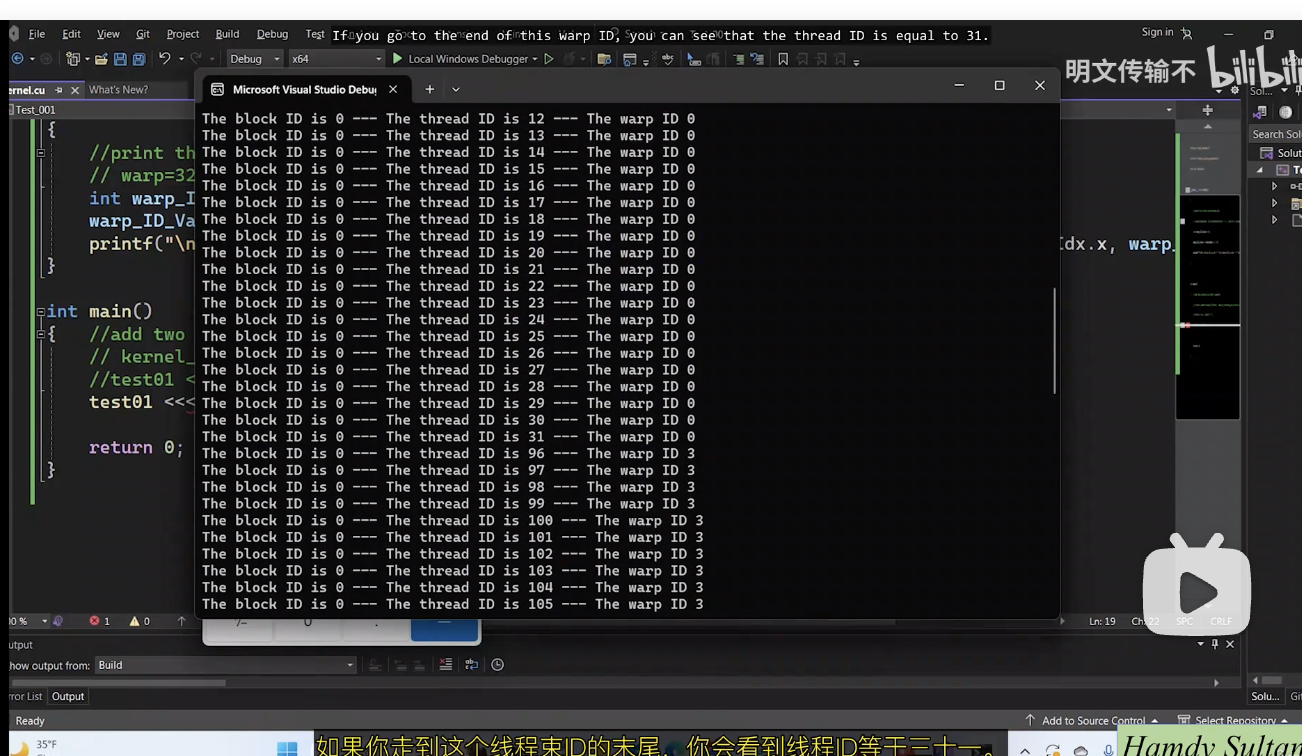
\includegraphics[width=0.75\linewidth]{resources/cuda-074.png}
    \caption{}
    \label{fig:placeholder}
\end{figure}

编译并运行后，输出显示两个块（块 ID 分别为 0 和 1）。关于线程束 ID，可以看到每个块都有线程束 ID 0 和线程束 ID 1。线程束 ID 0 在输出中出现了两次——因为线程束 ID 是\textbf{按块计算的}，而非针对整个 GPU。每个块都有自己独立的线程束编号，因此两个块各自拥有线程束 ID 0 和线程束 ID 1。

